\documentclass[xcolor={usenames,dvipsnames},handout]{beamer}
%\documentclass[draft]{beamer}


\usepackage[dvipsnames]{xcolor}



\usepackage[utf8]{inputenc}
\usepackage[T1]{fontenc}
\usetheme{MOKAbeamer}

%\usepackage[french]{babel}



\usepackage{tikz}

%\usepackage[draft]{animate}
\usepackage{animate}
\usepackage{ifthen}
\usepackage{filecontents}
\usepackage{stmaryrd}
\usepackage{listliketab}

\usepackage{multirow}

\usetikzlibrary{calc}
\usepackage{pifont}
\usepackage{mystyle}

\usepackage{tabularx}

\usepackage{algorithm,algorithmic}

\usepackage{standalone} % pour compiler les tikz -> input
\definecolor{vertsombre}{rgb}{0.0,0.5,0.0}
\usepackage{array}
\newcolumntype{M}{>{\centering\arraybackslash} m{0.5cm} }

\newcommand{\cyte}[1]{{\scriptsize\color{domcolor}#1}}
\newcommand{\cyteb}[1]{{\footnotesize\color{white}#1}}

%Pour ne pas compter les derniers slides
\newcommand{\backupbegin}{
   \newcounter{finalframe}
   \setcounter{finalframe}{\value{framenumber}}
}
\newcommand{\backupend}{
   \setcounter{framenumber}{\value{finalframe}}
}


%\newtheorem{theorem}{Theorem}[chapter]
%\newtheorem{lemma}[theorem]{Lemma}
\newtheorem{prop}[theorem]{Proposition}
%\newtheorem{corollary}[theorem]{Corollary}
%\newtheorem{definition}[theorem]{Definition \rm}
%\newtheorem{definition}[theorem]{Definition}
\newtheorem{remark}[theorem]{Remark}


%Debug boxes
\showboxdepth=5
\showboxbreadth=5


\newcommand{\nfb}[1]{\begin{frame}[allowframebreaks]#1\end{frame}}


\begin{document}
\title[]{Introduction to Machine learning}
\author[S.~Le Corff]{Sylvain Le Corff}
\date{}

\begin{frame}[plain]
\titlepage
\end{frame}


\begin{frame}{Logistic regression}
\tableofcontents
\end{frame}



\section{Mathematical framework}


\begin{frame}{Supervised  Learning}
\structure{{\bf Supervised Learning Framework}}

$\rightharpoondown$ \alert{Input} measurement $\textbf{X}  \in \mathcal{X}$ (often $\mathcal{X} \subset \mathbb{R}^d$).

$\rightharpoondown$  \alert{Output} measurement $Y \in \mathcal{Y}$.

$\rightharpoondown$  The joint distribution of $(\textbf{X},Y)$ is  \alert{unknown}.

$\rightharpoondown$  $Y \in \{1,\ldots,M\}$ (classification) or $Y \in \mathbb{R}^m$ (regression).


$\rightharpoondown$ A \alert{predictor} is a measurable function $f:\mathcal{X} \to \mathcal{Y}$.

\vspace{.5cm}

\structure{{\bf Training data}}

$\rightharpoondown$ i.i.d. with the same distribution as $(\textbf{X},Y)$:
$$\mathcal{D}_n=\{(\textbf{X}_1, Y_1),\ldots,(\textbf{X}_n, Y_n)\}\,.$$ 




\vspace{.5cm}

\structure{{\bf Goal}}

$\rightharpoondown$  Construct a \alert{good} predictor $\widehat{f}_n$ from the training data.

$\rightharpoondown$  Need to specify the meaning of good.

\end{frame}

\begin{frame}{Loss and Probabilistic Framework}
\structure{{\bf Loss function}}

$\rightharpoondown$ $\ell(Y,f(\textbf{X}))$: the goodness of the prediction of $Y$ by $f(\textbf{X})$.

$\rightharpoondown$ \alert{Prediction} loss: $\ell(Y,f(\textbf{X}))=\mathbf{1}_{Y\neq f(\textbf{X})}$.

$\rightharpoondown$  \alert{Quadratic} loss: $\ell(Y,\textbf{X})=\|Y-f(\textbf{X})\|_2^2$.

\vspace{.5cm}

\structure{{\bf Risk function}}

$\rightharpoondown$ Risk measured as the average loss:
	\[
	\alert{\mathcal{R}(f)=\E[\ell(Y,f(\textbf{X}))}]\,.
	\]

$\rightharpoondown$ \alert{Prediction} loss: $\E[\ell(Y,f(\textbf{X}))]=\mathbb{P}(Y\neq f(\textbf{X}))$.

$\rightharpoondown$ \alert{Quadratic} loss: $\E[\ell(Y,f(\textbf{X}))]=\E[\|Y-f(\textbf{X})\|_2^2]$.

\vspace{.3cm}

$\rightharpoondown$ {\color{Vert} \textbf{Beware:}}  As $\widehat{f}_n$ depends on $\mathcal{D}_n$, $\mathcal{R}(\widehat{f}_n)$ is a random variable!

\end{frame}



%\begin{frame}{Mathematical framework for today }
%\begin{block}{Supervised learning}
%Given observations, $d_n = \left\{ (x_1,y_1), (x_2,y_2), \hdots (x_n,y_n) \right\}$ we want to explain/predict outputs $y_i \in \Yc$ from inputs $x_i \in \Xc$.
%
%\textbf{\structure{Goal}}
%\begin{itemize}
%\item Explain/Learn connections between inputs $x_i$ and outputs $y_i$ ; 
%\item Predict the output $y$ for a new input $x\in \Xc$
%\end{itemize}
%\end{block}
%
%\pause
%To do so, we have to find a \structure{machine} or \structure{function} $f : \Xc \to \Yc$ such that 
%$$
%f(x_i) \simeq y_i , i= 1, \hdots , n.
%$$
%\pause
%\begin{exampleblock}{Jargon}
%\begin{itemize}
%\item When the output $y$ is continuous, $\leadsto$ regression problem
%\item When the output $y$ is categorical, $\leadsto$ classification problem
%\end{itemize}
%\end{exampleblock}
%\end{frame}



%\subsection{Linear and quadratic discriminant analysis}
%\subsection{Bayes classifier for multivariate normal distributions}

\begin{frame}{Binary classification}

\begin{block}{Bayes classifier} 
The \structure{Bayes classifier} $g^\star$ is defined as:
$$
g^{\star}(X) =
\left\{
	\begin{array}{cc}
		1 &\quad \text{if} \quad \P \left( Y=1 | X \right) > \P \left( Y=0 | X \right), \\
		0 &\quad \text{otherwise}. \hfill
	\end{array}
\right.
$$
Equivalently,
$$
g^{\star}(X) =
\left\{
	\begin{array}{cc}
		1 &\quad \text{if} \quad \P \left( Y=1 | X \right)> 1/2, \\
		0 &\quad \text{otherwise}, \hfill
	\end{array}
\right.
$$
\end{block}
\begin{lemma}
For any classification rule $g :  \R^d \to \{0,1\}$, one has
$$
\Rc(g^\star) \leq \Rc(g).
$$
\end{lemma}
\end{frame}

	
\begin{frame}{How to model the conditional law of $Y$?}
 In practice \alert{we do not know  the conditional law of $Y$ given $X$}. Several solutions to overcome this issue.


\vspace{.4cm}


\structure{{\bf Fully parametric modeling.}}
    
     Estimate the law of $(X,Y)$
      and use the \textbf{Bayes formula} to deduce an estimate of
      the conditional law of $Y$: \emph{LDA/QDA, Naive Bayes...}

\vspace{.3cm}

\structure{{\bf Parametric conditional modeling.}}
    
     Estimate the conditional law of
      $Y$ by a \textbf{parametric} law: \emph{linear regression, logistic regression, Feed Forward Neural Networks...}

\vspace{.3cm}

\structure{{\bf Nonparametric conditional modeling.}}
    
     Estimate the conditional  law of
      $Y$ by a \textbf{non parametric} estimate: \emph{kernel
        methods, nearest neighbors...}

 
\end{frame}





\section{Logistic regression}




\begin{frame}{Recall the linear model}
\begin{itemize}
\item In regression with $\Xc = \R^d$ , the linear model is the \structure{parametric reference model}.
\pause 
\item This model makes the assumption that the regression function is linear: for $1\leq i \leq n$
$$
Y =  X^\top \beta^\star +\varepsilon,
$$
with 
$$
\E [ \varepsilon| X ] = 0 \quad \text{and } \quad \V [ \varepsilon | X] = \sigma^2.
$$
\item Here, estimating the regression function is equivalent to estimate $\beta^\star \in \R^d$.

\vspace{.2cm}

{\color{Vert}Finite dimensional parametric model}
%$m^\star$ is characterized by the parameter $\beta^\star \in \R^d$ (finite dimension) \\ $\Rightarrow$ parametric model.  
\end{itemize} 
\end{frame}

\begin{frame}{ERM with quadratic loss} 


\begin{itemize}
\item The least squares estimates, i.e. the optimal solution of
$$
\min_{\beta \in \R^d} \widehat{\Rc}_n (\beta) = \min_{\beta \in \R^d} \frac{1}{n} \sum_{i=1}^n (Y_i - X_i^T \beta)^2
$$
with $Y\in\R^n$, $X\in \R^{n\times d}$ is given, \alert{if $X$ has full rank}, by
 
$$
\widehat{\beta}_n  = (X^\top X)^{-1} X^\top Y.
$$
\item  $m^\star: x \mapsto x^\top \beta^*$ is estimated by $\widehat{m}_n: x \mapsto  x^\top \widehat{\beta}_n$. 
\item Under some technical assumptions (see lectures of past year)
{\color{Vert}$$
\E [ \widehat{\beta}_n  ] = \beta^\star \quad \text{and} \quad \V (\widehat{\beta}_n   ) = \sigma^2 (X^\top X)^{-1} .
$$}
\item We deduce that, see \url{sylvainlc.github.io},
$$
\E \left[ \| \widehat{\beta}_n - \beta \|_2^2 \right] = O \left( \frac{1}{n} \right) \quad \text{and} \quad \E \left[ ( \hat{m}_n(x) - m^\star(x) )^2 \right] = O \left( \frac{1}{n} \right) 
$$
\end{itemize}
\end{frame}


\begin{frame}\frametitle{Fully parametric modeling - Discriminant Analysis}


In the LDA case, the classification rule is of the form:
\begin{equation*}
g^*(x) = 1 \Leftrightarrow \langle w,x \rangle + b \geqslant 0\,,
\end{equation*}
where \alert{$w$ and $b$ depends on the model parameters}.

\begin{center}
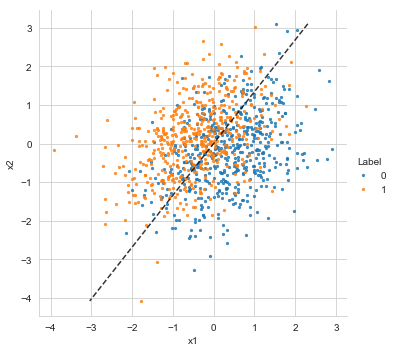
\includegraphics[width=5cm]{./logistic.png} 
\end{center}

$\rightharpoondown$ Relax the Gaussian assumption ? (\alert{logistic model, SVM}).

$\rightharpoondown$ Design  nonlinear classification rules ? (\alert{kernels, neural networks}).

\end{frame}

\begin{frame}{The logistic model}

\begin{itemize}
\item One of the most widely used classification algorithm.

%\item Logistic model is the "brother" of the linear model in the context of binary classification 
%($\Yc = \{0, 1\}$).

%\item We want to explain the label $Y$ based on $X$, we want to
%"regress" $Y$ on $X$.

\item It \structure{models the distribution of $Y$ given $X$}.
For $y\in \{0, 1\}$
$$
\P\left(  Y = 1 | X \right) = \sigma \left( X^\top w +b \right)
$$
where $w\in \R^d$ is a vector of model weights and $b\in\R$ is the
intercept, and where $\sigma:z \mapsto (1+ \mathrm{e}^{-z})$ is the \structure{sigmoid} function:
\end{itemize}

\begin{figure}[H]
\begin{center}
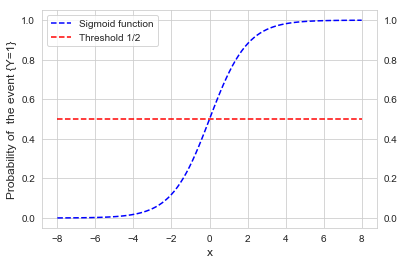
\includegraphics[height=3cm]{./sigmoid}
\caption{The sigmoid function}
\end{center}
\end{figure}

\end{frame}



\begin{frame}{Some comments on the logistic model}
\begin{itemize}
\item The sigmoid is a modelling choice to map $\R \to [0, 1]$ (to model a probability).
\item We could also consider
$$
\P\left(  Y = 1 | X\right) = F \left( X^\top w +b \right)
$$
\alert{for any distribution function $F$}. 
\item Another popular choice is the
Gaussian distribution
$$ F(z) = \P(\Nc(0,1) \leq  z),
$$
which leads to another loss called {\color{PineGreen}probit}.
\end{itemize}
\end{frame}

\begin{frame}{The logistic model}

\begin{itemize}
\item In the case of the sigmoid,
one has
\begin{align*}
\P\left(  Y = 1 | X \right) &= \frac{\exp (b+ w^\top X)}{1+ \exp(b+ w^\top X)} = \frac{1}{1+\exp(-(b+ w^\top X)) } \\
\P\left(  Y = 0 | X \right) &=  \frac{1}{1+\exp(b+ w^\top X) }
\end{align*}

\item However, the sigmoid choice has the following nice interpretation: an easy computation leads to
$$
\log \left( \frac{\P\left(  Y = 1 | X \right)}{\P\left(  Y = 0| X  \right)} \right) = X^\top w +b.
$$
\item This quantity is called the \structure{log-odd ratio}.
\end{itemize}
\end{frame}

\begin{frame}{The logistic model}

\begin{itemize}
\item Therefore, this model makes the assumption that \structure{(the logit transformation of) the probability $p(X)=\P\left(  Y = 1 | X \right)$  is linear}:
$$
\mathrm{logit} (p(X)) := \log\left( \frac{p(X)}{1-p(X)} \right) = X^\top w + b.
$$
\pause
\item Note that 
\begin{block}{}
$$
\P\left(  Y = 1 | X \right) \geq \P\left(  Y = 0 | X \right)
$$
\underline{if and only if}
$$
X^\top w + b \geq 0.
$$
\end{block}
\pause
This is a \structure{linear classification rule}, linear w.r.t.\ the considered features $x$!
\end{itemize}
\end{frame}


\begin{frame}{The logistic "regression"}
\begin{theorem}
%	Let us consider that we have $C=2$ classes.
%	Then, under assumption that logit-transformation is linear, we have
%	$$
%		(b^\star, w^\star) \in \argmin_{(b, w)\in\R^\times\R^d} \E \left[\log\left( 1 + \exp(-Y(b + w^\top X)) \right) \right].
%	$$
%	Let
%	$$
%		(\bar b, \bar w) \in \argmin_{(b, w)\in\R^\times\R^d} \E \left[\log\left( 1 + \exp(-Y(b + w^\top X)) \right) \right].
%	$$
%	Then, under assumption that the logit-transformation is linear,
%	a Bayes classifier is
%	$$
%		g^\star \colon x \in \R^d \mapsto
%		\left\{ \begin{array}{ll}
%			+1 & \text{if } \bar b + \bar w ^\top x > 0 \\
%			-1 & \text{otherwise}.
%		\end{array} \right.
%	$$
	Consider that the logit-transformation is linear with parameters $(b^\star, w^\star)$:
$$
\mathrm{logit} (p(X)) := \log\left( \frac{p(X)}{1-p(X)} \right) = f^\star(X) =  X^\top w^\star + b^\star.
$$
	%Let $f^\star \colon x \in \R^d \mapsto b^\star + (w^\star) ^\top x$.
	Then \alert{$f^\star$ is a minimizer of the risk}:
	$f \mapsto \E \left[\log\left( 1 + \exp(-Yf(X)) \right) \right]$ over all affine functions and
	$$
		g^\star \colon x \in \R^d \mapsto
		\left\{ \begin{array}{ll}
			1 & \text{if } f^\star(x) > 0 \\
			0 & \text{otherwise}
		\end{array} \right.
	$$
	is a Bayes classifier.
\end{theorem}
%\centering
%{\color{Vert} Proof on blackboard !}
\end{frame}


\begin{frame}{Estimation of $w$ and $b$}

 \alert{Parametric model} for the conditional law of $Y$ given $X$: $\P_{w,b}(Y|X)$.

%\vspace{.2cm}
%
%Data $(X_i , Y_i)_{1\leq i \leq n}$  i.i.d with the same distribution as $(X,Y)$.

\vspace{.2cm}

Compute estimators $\hat{w}$ and $\hat{b}$ by maximum likelihood estimation.

\vspace{.2cm}

Or equivalently, \alert{minimize the minus log-likelihood}: 
\structure{
$$
(w,b)\mapsto -n^{-1}\log \P_{w,b}(Y_{1:n}|X_{1:n}).
$$ }
More generally, when a model is used
\begin{center}
Goodness-of-fit = -log likelihood
\end{center}
The log function is used mainly since averages are easier to study (and compute) than products.
\end{frame}

\begin{frame}{Logistic regression - likelihood function}

$\rightharpoondown$   $\{(X_i,Y_i)\}_{1\leqslant i\leqslant n}$ are \alert{i.i.d. with the same distribution as $(X,Y)$}.

\vspace{.3cm}


{\bf\structure{Likelihood:}}

\begin{align*}
 \prod_{i=1}^n \P_{w,b}(Y_i | X_i) &= \prod_{i=1}^n \sigma(\langle w,X_i \rangle + b)^{Y_i} \big(1 - 
\sigma(\langle w,X_i \rangle + b) \big)^{1 - Y_i}\,, \\
& = \prod_{i=1}^n \sigma(\langle w,x_i \rangle + b)^{Y_i} 
\sigma(-\langle w,X_i \rangle - b)^{1 - Y_i}
\end{align*}
\smallskip

and the \alert{normalized negative loglikelihood} is written
\smallskip

\begin{equation*}
f(w,b) = \frac{1}{n}\sum_{i=1}^n \ell(Y_i, \langle w,X_i \rangle + b)\,.
\end{equation*}
\end{frame}


\begin{frame}{Logistic regression - likelihood function}
		
Compute $\hat w_n$ and $\hat b_n$ as follows:

\begin{align*}
(\hat w_n, \hat b_n) \in \argmin_{w \in \R^d, b \in \R}
\frac 1n \sum_{i=1}^n\left(-Y_i (X_i^\top w+ b) +  \log(1+ e^{X_i^\top w + b})\right)\,.
\end{align*}

\vspace{.3cm}

$\rightharpoondown$ It is an \textbf{average of losses}, one for each sample point.

$\rightharpoondown$ It is a \alert{convex and smooth problem}.


\medskip

Using the \textbf{\alert{logistic loss}} function
\smallskip 

\begin{equation*}
\ell: (y, y') \mapsto \log(1 + e^{-y y'}) 
\end{equation*}

yields

\begin{equation*}
(\hat w_n, \hat b_n) \in \argmin_{w \in \R^d, b \in \R}
\frac 1n \sum_{i=1}^n \ell(Y_i, \langle w,X_i \rangle + b)\,.
\end{equation*}
\end{frame}




\begin{frame}{Maximum likelihood estimate}
Assume for now that the intercept is 0. Then, the likelihood is,

$$
L_n(w)  =  \prod_{i=1}^n \left(\frac{e^{X_i^Tw}}{1+e^{X_i^T w}} \right)^{Y_i} \left(\frac{1}{1+e^{X_i^T w}} \right)^{1-Y_i} = \prod_{i=1}^n \left(\frac{e^{X_i^Tw Y_i}}{1+e^{X_i^T w}} \right)\,.
$$

And the \alert{negative $\log$-likelihood} is

\begin{align*}
\ell_n(w) = - \log(L_n(w)) =  \sum_{i=1}^n \left(-Y_i X_i^T w+ \log(1+ e^{X_i^Tw})\right)\,.
\end{align*}

{\bf\textcolor{violet}{Derivatives}}

%$$
%\nabla  \left(\log(L_n(\beta))\right)=   \left(\frac{\partial}{\partial \beta_0}(\beta),\cdots, \frac{\partial}{\partial \beta_d}(\beta)\right)\,. 
%$$

\begin{eqnarray*}
\frac{\partial \left(\log(L_n(w))\right)}{\partial w_j}&= &
\sum_{i=1}^n \left(Y_i X_{ij}
	- \frac{x_{ij} e^{X_i^T
	w}}{(1+ e^{X_i^T
	w})}   \right) \\
&=& \sum_{i=1}^n X_{ij} \left(Y_i - \sigma(\langle w,X_i \rangle)\right)\,.
\end{eqnarray*}

$\rightharpoondown$ \alert{No explicit solution} for the maximizer of the loglikelihood... Parameter estimate obtained using \alert{gradient based optimization} (see next lesson).

\end{frame}

\begin{frame}{Maximum likelihood estimate}
The negative loglikelihood
\begin{align*}
\ell_n(w) = - \log(L_n(w)) =  \sum_{i=1}^n \left(-Y_i X_i^T w+ \log(1+ e^{X_i^Tw})\right)\,.
\end{align*}

is minimized using a gradient descent algorithm. 

Starting with an \alert{initial estimate $w^{(0)}$}, for all $k\geqslant 1$, set
\begin{align*}
w^{(k)} = w^{(k-1)} - \eta_k \nabla \ell_n(w^{(k-1)})\,.
\end{align*}

\begin{center}
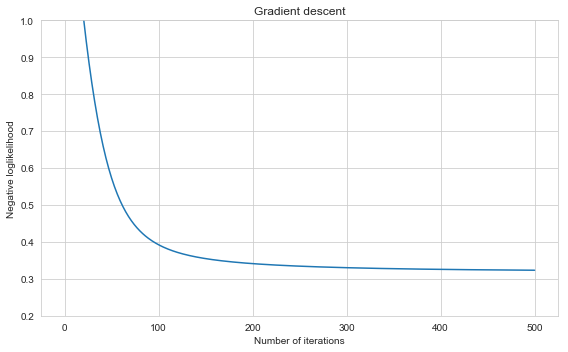
\includegraphics[width = 7cm]{gradient_descent.png}
\end{center}

\end{frame}

%\begin{frame}{Maximum likelihood estimate}
%Let $(w^*,b^*)$ be the parameter estimates \alert{after the gradient descent algorithm}.
%
%The usual logistic regression classifier is $f^*(X) = 1 \Leftrightarrow \mathbb{P}(Y = 1| X) >1/2$. 
%
%\textcolor{violet}{Sensitivity of the classifier to this threshold}: for each value $p^*\in(0,1)$ the ROC curve classifies individuals using $f^*(X) = 1 \Leftrightarrow\mathbb{P}(Y = 1| X) > p^*$ and plots the True positive rate as a function of the False positive rate. 
%
%
%\begin{center}
%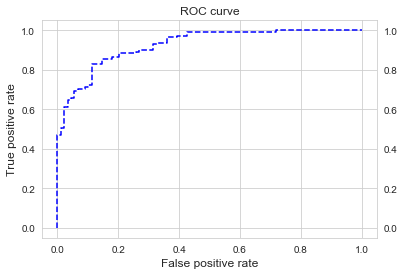
\includegraphics[width = 7cm]{roc_curve.png}
%\end{center}
%
%\end{frame}

\begin{frame}
The \alert{gradient of the negative loglikelihood} is, 

\begin{align*}
\nabla \ell_n(w) = - \sum_{i=1}^n Y_i X_i + \sum_{i=1}^n \frac{\exp(\langle X_{i},w\rangle)}{1  + \exp(\langle X_{i},w\rangle)} X_i\,.
\end{align*}

\vspace{.2cm}

On the other hand, for all $1\leqslant i \leqslant n$ and all $1 \leqslant j \leqslant d$,
\[
\partial_j \left( \frac{\exp(\langle X_{i},w\rangle)}{1  + \exp(\langle X_{i},w\rangle)} X_i \right) = \frac{\exp(\langle X_{i},w\rangle)}{(1  + \exp(\langle X_{i},w\rangle))^2} X_{ij}X_i\,,
\]
where $X_{ij}$ is the $j$th component of $X_i$. 

\vspace{.2cm}

Then, the \alert{Hessian matrix} is

%\[
%\big(H_n(w)\big)_{\ell j} = \sum_{i=1}^n \frac{\exp(\langle X_{i},w\rangle)}{(1  + \exp(\langle X_{i},w\rangle))^2} X_{ij}X_{i \ell}\,,
%\]
%that is,
%{\color{Vert}{
\begin{align*}
H_n(w) = \sum_{i=1}^n \frac{\exp(\langle X_{i},w\rangle)}{(1  + \exp(\langle X_{i},w\rangle))^2} X_{i} X^T_{i}\,.
\end{align*}
%}
%\vspace{.3cm}
%
%{\bf \textcolor{violet}{$H_n(\beta)$ is a semi positive definite matrix, which implies that $\ell_n(\beta)$ is convex}}.

\end{frame}

\begin{frame}{Asymptotic properties}


{\bf\textcolor{violet}{Assumptions}}

$\rightharpoondown$ \alert{$\widehat w_n\to w^*$ almost surely}. 

$\rightharpoondown$ There exists a continuous and nonsingular function $H$ such that \alert{$n^{-1}H_{n}(w)$ converges to $H(w)$}, uniformly in a ball around $w^*$.

\vspace{.5cm}

For all $t\in\R^d$, using a Taylor expansion,
\[
\mathbb{E} \left[ \exp\left( - \frac{1}{\sqrt{n}} \langle t, \nabla \ell_n(w^{\star}) \rangle \right) \right] \to_{n\to \infty}  \exp\Bigg( \frac{1}{2} t^T H(w^{\star}) t \Bigg)\,.
\]

Therefore, 
\begin{align*}
-\nabla \ell_n(w^{\star}) / \sqrt{n} \Rightarrow \mathcal{N}(0, H(w^{\star}))\,.
\end{align*}

\vspace{.5cm}

On the other hand, by \alert{Slutsky lemma}, 

\begin{align*}
\sqrt{n} (\widehat{w}_n - w^{\star}) \Rightarrow \mathcal{N}(0,  H(w^{\star})^{-1})\,.
\end{align*}

\end{frame}

\begin{frame}{Confidence interval}

$\rightharpoondown$ $\sqrt{n} ( \widehat{w}_j - w^{\star}_j) $ \alert{converges in distribution to a centered Gaussian random variable with variance $(H(w^{\star})^{-1})_{jj}$}.

\vspace{.3cm}

Almost surely, $\widehat{\sigma}_{n,j}^2 = (n H_n(\widehat{w}_n)^{-1})_{jj} \to_{n\to \infty} (H(w^{\star})^{-1})_{jj}$.

Then, 

\begin{align*}
\sqrt{\frac{n}{\widehat{\sigma}_{n,j}^2}} (\widehat{w}_{n,j} - \beta^{\star}_j ) \to_{n\to \infty} \mathcal{N}(0,1)\,.
\end{align*}

\vspace{.2cm}

An \alert{asymptotic confidence interval $\mathcal{I}_{n,\alpha}$ of level $1-\alpha$} is then 



\begin{align*}
\mathcal{I}_{n,\alpha} = \left[ \widehat{w}_{n,j} - z_{1-\alpha/2} \sqrt{\frac{\widehat{\sigma}^2_{n,j}}{n}}\,,\; \widehat{\beta}_{n,j} + z_{1-\alpha/2} \sqrt{\frac{\widehat{\sigma}^2_{n,j}}{n}}  \right]\,,
\end{align*}

\vspace{.2cm}
where $z_{1- \alpha/2}$ is the quantile of order $1- \alpha/2$ of $\mathcal{N}(0, 1)$.
\end{frame}


%\begin{frame}{Summary: LDA/QDA/Logistic reg}
%
%
% \textbf{Logistic regression} directly models the parameter of the distribution of \structure{$Y$ given $X$}.
%
%\begin{itemize}
%\item The \structure{logit transformation of the probability} $p(X)=\P\left(  Y = 1 | X \right)$  is \alert{linear}:
%$$
%\mathrm{logit} (p(X)) := \log\left( \frac{p(X)}{1-p(X)} \right) = X^\top w + b.
%$$
%\end{itemize}
%
%\textbf{Linear discriminant analysis} do the opposite. 
%
%\begin{itemize}
%\item It models the distributions of \structure{$X$ given $Y = j$} for $j = 1,...,M$ by Gaussian distributions $f_j(x)$,
%\item  The posterior distribution of $Y$ given $X$ can be computed with Bayes formula:
%$$
%\P \left( Y =j | X \right) = \frac{\pi_j f_j(X) }{\sum_\ell^M \pi_\ell f_\ell(X)},
%$$
%with $\pi_j = \P(Y=j)$.
%\end{itemize}
%
%\end{frame}
%
%\begin{frame}{Summary: LDA/QDA/Logistic reg}
%
%\begin{itemize}
%\item Classification rule: we choose the group which maximizes these probabilities
%$\hat{g}(X)=k$ if and only if $\P(Y=k|X)\geq \P(Y=j|X), \forall j \neq k$.
%\item Boundary between 2 groups: set of points x such that 
%$$\P (Y =k|X )=\P(Y =j|X )$$
%i.e.\
%\begin{align*}
%0 &= \log\left(\frac{\P (Y =k|X)}{\P(Y =j|X)} \right) =  \log\frac{f_k(X)}{f_j(X)}+ 	\log\frac{\pi_k}{\pi_j} \\
%&= \log\frac{\pi_k}{\pi_j} + \frac{1}{2} (\mu_k + \mu_j)^T \Sigma^{-1} (\mu_k - \mu_j) + X^\top \Sigma^{-1} (\mu_k - \mu_j)
%\end{align*}
%which is \alert{linear} in $x$!
%\end{itemize}
%
%\end{frame}

%
%\begin{frame}{Regression and linear model}
%\begin{remark}  
%\begin{itemize}
%\item Least squares estimates achieve the parametric rate $O(1/n)$.
%\item Moreover, if errors terms $(\varepsilon_i)_i$ are Gaussian, we can compute the distribution of the least squares estimates (confidence intervals, test statistics...).
%\end{itemize}
%\end{remark}
%
%\vspace{.3cm}
%
%{\color{Vert} See \href{https://sylvainlc.github.io/}{[Lecture notes on statistical learning, Chapter 2]} for additional details (Ridge/Lasso  regression)...}
%\end{frame}
%
%
%
%\begin{frame}{Going beyond: the logistic model}
%
%\begin{itemize}
%\item One of the most widely used classification algorithm in the context of binary classification 
%($\Yc = \{-1, 1\}$).
%
%\item We want to explain the label $Y$ based on $X$, we want to
%"regress" $Y$ on $X$.
%
%\item It \structure{models the distribution of $Y$ given $X$}.
%For $y\in \{-1, 1\}$
%$$
%\P\left(  Y = 1 | X =x \right) = \sigma \left( x^T w +b \right)
%$$
%where $w\in \R^d$ is a vector of model weights and $b\in\R$ is the
%intercept, and where $\sigma$ is the \structure{sigmoid} function:
%\end{itemize}
%%\begin{minipage}{0.45\textwidth}
%%$$
%%\sigma(z) = \frac{1}{1+e^{-z}}. 
%%$$
%%\end{minipage}
%%\begin{minipage}{0.35\textwidth}
%%\begin{figure}[H]
%%\begin{center}
%%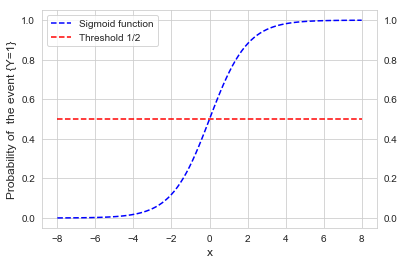
\includegraphics[height=2cm]{./sigmoid}
%%%\caption{The sigmoid function}
%%\end{center}
%%\end{figure}
%%\end{minipage}
%\end{frame}
%
%\begin{frame}{Going beyond: the logistic model}
%\begin{figure}[H]
%\begin{center}
%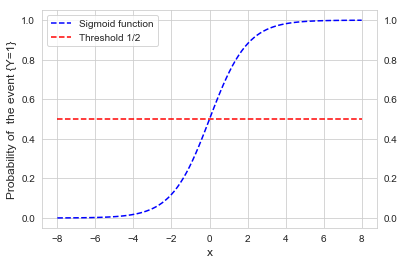
\includegraphics[scale = .6]{./sigmoid}
%%\caption{The sigmoid function}
%\end{center}
%\end{figure}
%\end{frame}
%
%
%\begin{frame}{Some comments on the logistic model}
%\begin{itemize}
%\item The sigmoid choice really is a choice. It is a modelling choice.
%\item It is a way to map $\R \to [0, 1]$ (we want to model a probability).
%\item We could also consider
%$$
%\P\left(  Y = 1 | X \right) = F \left( X^\top w +b \right)
%$$
%for any distribution function $F$. 
%\pause
%\item Another popular choice is the
%Gaussian distribution
%$$ F(z) = \P(\Nc(0,1) \leq  z),
%$$
%which leads to another loss called {\color{PineGreen}probit}.
%\end{itemize}
%\end{frame}
%
%\begin{frame}{The logistic model}
%
%\begin{itemize}
%\item In the case of the sigmoid,
%one has
%\begin{align*}
%\P\left(  Y = 1 | X  \right) &= \frac{\exp (b+ w^\top X)}{1+ \exp(b+ w^\top X)} = \frac{1}{1+\exp(-(b+ w^\top X)) } \\
%\P\left(  Y = - 1 | X \right) &=  \frac{1}{1+\exp(b+ w^\top X) }
%\end{align*}
%
%\item However, the sigmoid choice has the following nice interpretation: an easy computation leads to
%$$
%\log \left( \frac{\P\left(  Y = 1 | X  \right)}{\P\left(  Y = -1 | X \right)} \right) = X^\top w +b.
%$$
%\item This quantity is called the \structure{log-odd ratio}.
%\end{itemize}
%\end{frame}
%
%\begin{frame}{The logistic model}
%
%\begin{itemize}
%\item Therefore, this model makes the assumption that \structure{(the logit transformation of) the probability $p(X)=\P\left(  Y = 1 | X  \right)$  is linear}:
%$$
%\mathrm{logit} (p(X)) := \log\left( \frac{p(X)}{1-p(X)} \right) = X^\top w + b.
%$$
%\pause
%\item Note that 
%\begin{block}{}
%$$
%\P\left(  Y = 1 | X  \right) \geq \P\left(  Y = -1 | X  \right)
%$$
%\underline{\textbf{iff}}
%$$
%X^\top w + b \geq 0.
%$$
%\end{block}
%\pause
%This is a \structure{linear classification rule}, linear w.r.t.\ the considered features $x$!
%\end{itemize}
%\end{frame}
%
%
%\begin{frame}{The logistic "regression"}
%\begin{theorem}
%%	Let us consider that we have $C=2$ classes.
%%	Then, under assumption that logit-transformation is linear, we have
%%	$$
%%		(b^\star, w^\star) \in \argmin_{(b, w)\in\R^\times\R^d} \E \left[\log\left( 1 + \exp(-Y(b + w^\top X)) \right) \right].
%%	$$
%%	Let
%%	$$
%%		(\bar b, \bar w) \in \argmin_{(b, w)\in\R^\times\R^d} \E \left[\log\left( 1 + \exp(-Y(b + w^\top X)) \right) \right].
%%	$$
%%	Then, under assumption that the logit-transformation is linear,
%%	a Bayes classifier is
%%	$$
%%		g^\star \colon x \in \R^d \mapsto
%%		\left\{ \begin{array}{ll}
%%			+1 & \text{if } \bar b + \bar w ^\top x > 0 \\
%%			-1 & \text{otherwise}.
%%		\end{array} \right.
%%	$$
%	Let us consider that $C=2$ and that the logit-transformation is linear with parameters $(b^\star, w^\star)$.
%	Let $f^\star \colon x \in \R^d \mapsto b^\star + (w^\star) ^\top x$.
%
%	Then $f^\star$ is a minimizer of the risk functional
%	$f \mapsto \E \left[\log\left( 1 + \exp(-Yf(X)) \right) \right]$ over all affine functions and
%	$$
%		g^\star \colon x \in \R^d \mapsto
%		\left\{ \begin{array}{ll}
%			+1 & \text{if } f^\star(x) > 0 \\
%			-1 & \text{otherwise}
%		\end{array} \right.
%	$$
%	is a Bayes classifier.
%\end{theorem}
%\end{frame}
%
%\begin{frame}[allowframebreaks]{Proof}
%
%	First, let us remark that $g^\star$, as previously defined, is a Bayes classifier, since $f^\star(x) > 0$ if and only if $\P(Y=+1 | X=x) > \P(Y=-1 | X=x)$.
%
%	Second, without loss of generality, we consider that $b$ vanishes and we denote $\ell \colon (x, y, w) \mapsto \log\left( 1 + \exp(-y w^\top x) \right)$.
%	Then, $\forall (x, y) \in \R^d \times \R$,
%	$$
%		\nabla_{w}{\ell}(x, y, w)
%		= - \frac{y}{1+\exp(y w^\top x)} x
%		= - \frac{y \exp(-y w^\top x)}{1+\exp(-y w^\top x)} x.
%	$$
%	Thus, since $\nabla_{w}{\ell}$ is Lebesgue-measurable, we can switch derivative and integral, leading to:
%	\begin{align*}
%		\nabla_w & {\E(\ell(X, Y, w)|X)}\\
%		&= \P(Y=+1 | X) \nabla_w{\psi}(X, 1, w) + \P(Y=-1 | X) \nabla_w{\psi}(X, -1, w) \\
%		&= - \frac{\exp((w^\star)^\top x)}{1+\exp((w^\star)^\top x)} \frac{1}{1+\exp(w^\top X)} X \\
%		&\quad +
%		\frac{1}{1+\exp((w^\star)^\top x)} \frac{\exp(w^\top X)}{1+\exp(w^\top X)} X.
%	\end{align*}
%	Thus, $\nabla_{w}{\E(\ell(X, Y, w^\star)|X)} = 0$ and $\nabla_{w}{\E(\ell(X, Y, w^\star))} = 0$.
%	Since $\ell$ is convex in $w$, this proves that $w^\star$ is a minimizer of $\E(\ell(X, Y, \cdot))$.
%\end{frame}
%
%\begin{frame}{Estimation of $w$ and $b$}
%
%\begin{itemize}
%\item We have a model for the conditional law of $Y$ given $X$.
%\item Data $(X_i , X_i)$ is assumed i.i.d with the same distribution as $(X,Y)$
%\item Compute estimators $\hat{w}$ and $\hat{b}$ by maximum likelihood estimation
%\item Or equivalently, minimize the minus log-likelihood.
%\item  More generally, when a model is used
%\begin{center}
%Goodness-of-fit = -log likelihood
%\end{center}
%log is used mainly since averages are easier to study (and compute) than products
%\end{itemize}  
%\end{frame}
%
%
%\begin{frame}{The logistic "regression"}
%By introducing the logistic loss function
%$$
%\ell (y , y') = \log (1+e^{-yy'} ),
%$$
%then
%$$
%\hat{w}, \hat{b} \in \argmin_{w\in \R^d \atop b \in \R} \frac{1}{n} \sum_{i=1}^n \ell (y_i , x_i^T w+b).
%$$
%
%\begin{itemize}
%\item It is a convex and smooth problem
%\item Many ways to find an approximate minimizer 
%\item Efficient convex optimization algorithms (more on that later)
%\end{itemize}
%\end{frame}
%
%\begin{frame}{But...}
%\begin{remark}
%However, if there exists a separating hyperplane for $(X_i,Y_i)_{1\leq i \leq n}$ i.e.\ if there exists $(b_0,w_0)$ such that
%$$
%\forall i=1,\hdots , n , \qquad Y_i (w_0^T X_i +b_0) >0,
%$$
%then there is no minimizer of the negative log-likelihood! Convince yourself! 
%\end{remark}
%\end{frame}
%
%\begin{frame}{Summary: LDA/QDA/Logistic reg}
%
%
% \textbf{Logistic regression} directly models the parameter of the distribution of \structure{$Y|X = x$}
% \pause
%\begin{itemize}
%\item The \structure{logit transformation of the probability} $p(x)=\P\left(  Y = 1 | X =x \right)$  is \alert{linear}:
%$$
%\mathrm{logit} (p(x)) := \log\left( \frac{p(x)}{1-p(x)} \right) = x^T w + b.
%$$
%\end{itemize}
%
%\textbf{Linear discriminant analysis} do the opposite. 
%\pause
%\begin{itemize}
%\item It models the distributions of \structure{$X|Y = j$} for $j = 1,...,C$ by Gaussian distributions $f_j(x)$,
%\item  The posterior distribution $Y|X = x$ can be computed with Bayes formula:
%$$
%\P \left( Y =j | X=x \right) = \frac{\pi_j f_j(x) }{\sum_\ell^C \pi_\ell f_\ell(x)},
%$$
%with $\pi_j = \P(Y=j)$.
%\end{itemize}
%
%\end{frame}
%
%\begin{frame}{Summary: LDA/QDA/Logistic reg}
%
%\begin{itemize}
%\item Classification rule: we choose the group which maximizes these probabilities
%$\hat{g}(x)=k$ if and only if $\P(Y=k|X=x)\geq \P(Y=j|X=x), \forall j \neq k$.
%\item Boundary between 2 groups: set of points x such that 
%$$\P (Y =k|X =x)=\P(Y =j|X =x)$$
%i.e.\
%\begin{align*}
%0 &= \log\left(\frac{\P (Y =k|X =x)}{\P(Y =j|X =x)} \right) =  \log\frac{f_k(x)}{f_j(x)}+ 	\log\frac{\pi_k}{\pi_j} \\
%&= \log\frac{\pi_k}{\pi_j} + \frac{1}{2} (\mu_k + \mu_j)^T \Sigma^{-1} (\mu_k - \mu_j) + x^T \Sigma^{-1} (\mu_k - \mu_j)
%\end{align*}
%which is \alert{linear} in $x$!
%\end{itemize}
%
%\end{frame}
%
%
%
%
%
%%\section{Convex losses}
%%
%%\begin{frame}{Convexification}
%%
%%\begin{itemize}
%%\item The classification loss $\one_{g(x)\neq y}$ can be difficult to optimize (NP-hard).
%%\item The idea is to smooth the indicator $(g(x),y)\mapsto \one_{g(x)\neq y}$.
%%\item In the case of binary classification between $-1$ and $1$, one has
%%$$
%%\E \one_{Yf(X)<0} \leq \Rc (f) \leq \E \one_{Yf(X) \leq 0}
%%$$
%%so one can rewrite the indicator as follows
%%$(g(x),y)\mapsto \one_{g(x) y\leq 0}$
%%Then we want to bound it from above with a convex function of $yg(x) (=yy')$.
%%\end{itemize}
%%\end{frame}
%%
%%
%%\begin{frame}{Typical choices for convex loss functions}
%%\begin{itemize}
%%\item Hinge loss (SVM) : $\ell(y,y') = (1-yy')_+$
%%\item Quadratic Hinge loss :  $\ell(y,y') = \frac{1}{2}(1-yy')_+^2$
%%\item Huber loss : $ \ell(y,y') = -4 yy'\one_{yy'<-1}+  (1-yy')_+^2\one_{yy'\geq-1}$
%%\item Logit loss : $\ell (y , y') = \log (1+e^{-yy'} )$
%%\end{itemize}
%%
%%\begin{figure}[H]
%%\begin{center}
%%\includegraphics[height=6cm]{notes/img/convex_losses}
%%\end{center}
%%\caption{Examples of convex losses that all bound from above the $0-1$ function}
%%\end{figure}
%%
%%\underline{Exercise:}
%%Compute the biconjugate of the 0-1 loss.
%%\end{frame}
%%
%%
%%\begin{frame}
%%\begin{alertblock}{Question} 
%%What do we loose by convexifying the risk?
%%\end{alertblock}
%%\pause
%%\begin{itemize}
%%\item Let us consider $\phi : \R \to \R_+$ a loss function such that $\phi$ is \structure{strictly decreasing strictly
%%convex, differentiable,}
%%$$\phi(0) = 1 \qquad \lim_{x\to \infty} \phi(x)=0.$$
%%\pause
%%\item One can then define the associated risk and its empirical version:
%%$$
%%A(f) = \E [ \phi(Yf(X)) ]\quad \text{and} \quad 
%%A_n(f) = \frac{1}{n}\sum_{i=1}^n\phi (Y_if(X_i)).
%%$$
%%\end{itemize}
%%\end{frame}
%%
%%
%%\subsection{About the risk minimizer}
%%
%%\begin{frame}{About the "true" risk minimizer}
%%
%%
%%\begin{alertblock}{Question}
%%What is $f^\star = \argmin_f A(f)$ for $\phi$ strictly convex and differentiable? 
%%\end{alertblock}
%%
%%\pause 
%%\begin{itemize}
%%\item Clearly, since $Y\in \{-1,1\}$,
%%$$\E[ \phi(Yf(X))  |X=x ]=r(x)\phi (f(x))+(1-r(x))\phi(-f(x)), $$
%%(recall that $r(x) = \P(Y=1|X=x)$)
%%\pause 
%%\item  Consequence: $f^\star(x) = \argmin_\alpha h_{r(x)}(\alpha)$, where
%%$$h_r(\alpha)=r \phi(\alpha)+(1-r) \phi(-\alpha), \quad r\in  [0,1].
%%$$
%%\pause 
%%\item  Note: $h_r$ is strictly convex and therefore $f^\star$ is well defined.
%%\item The minimum is achieved for $h_r'(\alpha)=0$, i.e.\
%%$$
%%\frac{r}{1-r} = \frac{\phi'(-\alpha)}{\phi'(\alpha)}.
%%$$
%%\end{itemize}
%%\end{frame}
%%
%%\begin{frame}{About the "true" risk minimizer}
%%\begin{itemize}
%%\item Since $\phi'$ is strictly increasing, the solution is positive if and only if
%%$r > 1/2$
%%\item Conclusion: $f^\star (x)>0$ iff $r(x) = \P(Y=1|X=x)>1/2$
%%\item This is the \alert{Bayes classifier}!
%%$$
%%2 \one_{f^\star(x) >0} -1.
%%$$
%%\item Examples:
%%\begin{itemize}
%%\item $\phi(x) = e^{-x} \quad \Rightarrow \quad f^\star(x)=\frac{1}{2}\log(r(x)/(1-r(x))$
%%\item $\phi(x) = \text{hinge loss} \quad \Rightarrow \quad f^\star(x)= 2 \one_{r(x) >0} -1.$ the Bayes classifier itself!
%%\end{itemize}
%%\end{itemize}
%%\end{frame}
%%
%%
%%\subsection{Connection between 0-1 function and $\phi$-risk}
%%
%%\begin{frame}{Connection between 0-1 function and $\phi$-risk}
%%
%%\begin{exampleblock}{Objective}
%%\begin{itemize}
%%\item Connect $\Rc(f)-\Rc^\star$ with $A(f)-A^\star$.
%%\item Tool: $H : [0,1] \to \R$ defined by $H(r)= \inf_\alpha h_r(\alpha)$
%%\end{itemize}
%%\end{exampleblock}
%%
%%\pause
%%
%%\begin{lemma}
%%Let $\phi$ be a convex loss function such that the following hold:
%%\begin{enumerate}[(i)]
%%\item $f^\star>0$ iff $r(x)>1/2$
%%\item There exist constants $c\geq 0$ and $s\geq 1$ satisfying
%%$$
%%\left|\frac{1}{2} - r \right|^s \leq c^s(1-H(r)),\quad  r\in[0,1].
%%$$
%%Then, for any function $f : \R^d \to \R$,
%%$$
%%\Rc(f) - \Rc^\star \leq 2c (A(f) - A^\star)^{1/s}.
%%$$
%%\end{enumerate}
%%\end{lemma}
%%\end{frame}
%%
%%\begin{frame}{Connection between 0-1 function and $\phi$-risk}
%%$H$ can be evaluated for different losses:
%%\begin{itemize}
%%\item \structure{Exponential}: $H(r) = 2 \sqrt{r(1-r)}$
%%\item \structure{Logit}: $H(r) = -r\log_2 r-(1-r)\log_2(1-r)$
%%\item In both cases, $c =1/\sqrt{2}$ and $s=2$.
%%\item \structure{Hinge}: $H(r) =2 \min (r, 1-r) $, $\rightsquigarrow$ $c=1/2$ and $s=1$.
%%\end{itemize}
%%
%%$$
%%\Rc(f) - \Rc^\star \leq 2c (A(f) - A^\star)^{1/s}.
%%$$
%%
%%\end{frame}
%%
%%
%%
%%\subsection{Excess risk of convex minimizers}
%%
%%\begin{frame}{Excess risk of convex minimizers}
%%Consider the class
%%$
%%\Cc = \text{ a class of } \pm 1 \text{base classifiers} , 
%%$
%%and 
%%$$
%%\Fc_\lambda = 
%%\left\{ 
%%f = \sum_{j=1}^N c_j g_j : N \in \N, g_1,\hdots , g_N \in \Cc, \sum_{j=1}^N |c_j| = \lambda
%%\right\}
%%$$
%%\begin{theorem}
%%Let $f_n^{\star}\in {\arg\min}_{f \in  \Fc_{\lambda}} A_n(f)$, using either the \structure{exponential} or the \structure{logit} loss function, and let $\delta \in (0,1)$. Then, with probability at least $1-\delta$,
%%\begin{align*}
%%\Rc(f_n^{\star})-\Rc^{\star} \leq & 2 \bigg (8L_{\phi}\lambda \sqrt{\frac{VC_{\Cc}\log(n+1)}{n}}+B\sqrt{\frac{\log(1/\delta)}{2n}}\bigg)^{1/2}\\
%%& \qquad \qquad \qquad +\sqrt{2} \left( \inf_{f\in  \Fc_{\lambda}}A(f)-A^{\star}\right)^{1/2}.
%%\end{align*}
%%\end{theorem}
%%\end{frame}
%%\begin{frame}[allowframebreaks]{Proof}
%%
%%We have
%%\begin{align*}
%%\Rc(f_n^{\star})-\Rc^{\star} &\leq \sqrt 2 (A(f_n^{\star})-A^{\star})^{1/2}\\
%%&\leq \sqrt 2 \big(A(f_n^{\star})-\inf_{f \in \Fc_{\lambda}} A(f)\big)^{1/2}+\sqrt 2 \big(\inf_{f \in \mathscr F_{\lambda}} A(f)-A^{\star}\big)^{1/2}\\
%%& \leq 2 \big (\sup_{f \in \Fc_{\lambda}} |A_n(f)-A(f)|\big)^{1/2}+\sqrt 2 \big(\inf_{f \in \Fc_{\lambda}} A(f)-A^{\star}\big)^{1/2}\\
%%&\leq 2 \bigg (8L_{\phi}\lambda \sqrt{\frac{VC_{\Cc}\log(n+1)}{n}}+B\sqrt{\frac{\log(1/\delta)}{2n}}\bigg)^{1/2} \\
%%&\qquad \qquad  +\sqrt{2}\big(\inf_{f\in \Fc_{\lambda}}A(f)-A^{\star}\big)^{1/2}
%%\end{align*}
%%with probability at least $\delta$. At the last step we used the same bound for $\sup_{f \in \Fc_{\lambda}} |A_n(f)-A(f)|$ as in the {\large \color{WildStrawberry} to-do-list}.
%%\end{frame}
%%
%%\begin{frame}{Excess risk of convex minimizers}
%%\begin{align*}
%%\Rc(f_n^{\star})-\Rc^{\star} \leq & 2 \bigg (8L_{\phi}\lambda \sqrt{\frac{VC_{\Cc}\log(n+1)}{n}}+B\sqrt{\frac{\log(1/\delta)}{2n}}\bigg)^{1/2}\\
%%& \qquad \qquad \qquad +\sqrt{2} \left( \inf_{f\in  \Fc_{\lambda}}A(f)-A^{\star}\right)^{1/2}.
%%\end{align*}
%%Note that for
%%\begin{itemize}
%%\item Exponential: $L_\phi = e^\lambda$ and $B = e^\lambda$.
%%\item Logit: $L_\phi = 1/\log(2)$ and $B = \log_2(1+e^\lambda)$.
%%\item If $\inf A(f)-A^\star=0$, then $\Rc(f)-\Rc^\star= O \left(\sqrt{ \frac{log(n)}{n} }\right)$
%%\item The exponent in the rate is dimension-free!
%%\item Convex optimization, nous voil\`a! 
%%\item And also boosting algorithms
%%\end{itemize}
%%
%%\end{frame}
%%
%%
%%\begin{frame}{Epilog on convexification}
%%
%%\begin{block}{Take-home message}
%%\begin{itemize}
%%\item By studying a convex surrogate risk, we control the approximation error
%%$$
%%\Rc(f_n^{\star})-\Rc^{\star}
%%$$
%%\end{itemize}
%%\end{block}
%%
%%\begin{itemize}
%%\item[-] Statistics for high-dimensional data, \\
%%by P. Bühlmann \& S. Van de Geer
%%\item[-] Convexity,classification, and risk bounds, \\
%%by 
%%P. Bartlett,  M. Jordan, J. McAuliffe
%%\end{itemize}
%%\end{frame}
%%
%%
%%%\section{Linear Support Vector Machine (SVM)}
%%%
%%%
%%%\begin{frame}{Linear Support Vector Machine (SVM)}
%%% \begin{itemize}
%%%    \item Binary classification problem
%%%    \item We observe a training dataset of pairs $(x_i, y_i)$ for $i=1, \ldots, n$
%%%    \item Features $x_i \in \R^d$ and labels $y_i \in \{ -1, 1 \}$
%%%    \item Aim is to learn a classification rule that \textbf{generalizes} well
%%%    \item Given a features vector $x \in \R^d$, we want to predict the label $y$ 
%%%    \item Without \textbf{overfitting}
%%%  \end{itemize}
%%%\end{frame}
%%%
%%%\subsection{Preliminary}
%%%
%%%\begin{frame}{Linear classification}
%%%  Why?
%%%  \begin{itemize}
%%%    \item It's simple!
%%%    \item On very large datasets ($n$ is large, say $n \geq 10^7$), no other choice (training complexity)
%%%    \item Big data paradigm: lots of data $\Rightarrow$ simple methods are enough
%%%  \end{itemize}
%%%
%%%  % What is a linear classifier
%%%  % \begin{itemize}
%%%  % \item Using training data $(x_1, y_1), \ldots, (x_n, y_n)$,
%%%  %   construct a decision rule $f$ that predict the label $\hat y$ of a
%%%  %   new data point $x$    
%%%  % \item We saw that the logistic classifier is linear:
%%%  %   where $\sign z = 1$ if $z > 0$ and $\sign z = -1$ if $z < 0$, and
%%%  %   where $\hat \beta \in \R^d$ and $\hat b \in \R$ is the intercept
%%%  % \item The aim of linear classification is to find $\hat \theta$ and
%%%  %   $\hat b$ using the training data
%%%  % \end{itemize}
%%%
%%%  \medskip
%%%
%%%
%%%  
%%%  \begin{block}{A linear classifier}
%%%  
%%%  \begin{tabular}[htbp]{cc}    
%%%    \begin{minipage}[htbp]{.5\linewidth}
%%%      \vspace{0.2cm}
%%%      \begin{center}
%%%  				\includegraphics[width=5cm]{notes/img/SVM/lda_binary}
%%%      \end{center}
%%%    \end{minipage}
%%%    &
%%%    \begin{minipage}[htbp]{.5\linewidth}
%%%      Learn $\hat w \in \R^d$ and $\hat b$ s.t.\       
%%%      \begin{equation*}
%%%        \hat y = \sign(\langle {x, \hat w} \rangle + \hat b)
%%%      \end{equation*}
%%%      is a good classifier
%%%    \end{minipage}
%%%	\end{tabular}
%%%  \end{block}
%%%\end{frame}
%%%
%%%
%%%%\subsection{Linearly separable data}
%%%
%%%
%%%
%%%  \begin{frame}{Preliminary definitions}
%%%  
%%%  \begin{exampleblock}{}
%%%A dataset is {\color{Vert} linearly separable} if we can find an hyperplane $H$ that puts 
%%%\begin{itemize}
%%%  \item Points $x_i \in \R^d$ such that $y_i = 1$ on one side of the hyperplane
%%%  \item Points $x_i \in \R^d$ such that $y_i = -1$ on the other
%%%  \item $H$ do not pass through a point $x_i$
%%%\end{itemize}
%%%\end{exampleblock}
%%%
%%%\begin{center}
%%%  \includegraphics[width=0.5\textwidth]{notes/img/SVM/hyperplane.png}
%%%\end{center}
%%%\end{frame}
%%%
%%%
%%%
%%%\begin{frame}{Preliminary definitions}
%%%\begin{exampleblock}{}
%%%  An {\color{Vert}hyperplane }
%%%  \begin{equation*}
%%%      H = \{ x \in \R^d : w^T x + b = 0 \}
%%%  \end{equation*}
%%%  is a translation of a set of vectors orthogonal to $w$
%%%  \begin{itemize}
%%%    \item $w \in \R^d$ is a non-zero vector normal to the hyperplane
%%%    \item $b \in \R$ is a scalar 
%%%  \end{itemize}
%%% \end{exampleblock}
%%%  
%%%  
%%%    Definition of $H$ is invariant by multiplication of $w$ and $b$ by a non-zero scalar
%%%\end{frame}
%%%
%%%
%%%
%%%
%%%
%%%
%%%\begin{frame}{Canonical hyperplane}
%%%
%%%  If $H$ do not pass through any sample point $x_i$, we can scale $w$ and $b$ so that
%%%  \begin{equation*}
%%%    \min_{(x, y) \in D_n} |w^T x + b| = 1
%%%  \end{equation*}
%%%    For such $w$ and $b$, we call $H$ the {\color{Vert}canonical} hyperplane
%%%    
%%%    
%%%  \begin{figure}
%%%  \begin{center}
%%%    \includegraphics[width=0.5\textwidth]{notes/img/SVM/canonical_hyperplane.png}
%%%    \caption{The marginal hyperplanes are the hyperplanes parallel to the separating hyperplane and passing through the closest points on the negative or positive sides.}
%%%  \end{center}
%%%  \end{figure}
%%%
%%%
%%%\end{frame}
%%%
%%%
%%%\begin{frame}{The margin}
%%%  The distance of any point $x' \in \R^d$ to $H$ is given by
%%%  \begin{equation*}
%%%    \frac{|\langle {w, x'} \rangle  + b|}{\norm{w}}
%%%  \end{equation*}
%%%
%%%\begin{exampleblock}{}
%%%  So, if $H$ is a canonical hyperplane, its {\color{Vert}margin} is given by
%%%  \begin{equation*}
%%%    \min_{(x, y) \in D_n}   \frac{|w^T x + b|}{\norm{w}} 
%%%    = \frac{1}{\norm{w}}.
%%%  \end{equation*}
%%% \end{exampleblock}
%%%
%%%  \begin{center}
%%%    \includegraphics[width=6cm]{notes/img/SVM/margin}
%%%  \end{center}
%%%
%%%\end{frame}
%%%
%%%
%%%
%%%\begin{frame}{Summary}
%%%If $\Dc_n$ is strictly \structure{linearly separable}, we can find a \structure{canonical separating hyperplane} 
%%%\begin{equation*}
%%%  H = \{ x \in \R^d : w^T x + b = 0 \}.
%%%\end{equation*}
%%%that satisfies
%%%\begin{equation*}
%%%  |\langle {w, x_i} \rangle  + b| \geq 1 \; \text{ for any } \; i=1, \ldots, n,
%%%\end{equation*}
%%%which entails that a point $x_i$ is correctly classified if
%%%\begin{equation*}
%%%  y_i (\langle {x_i, w} \rangle  + b) \geq 1.
%%%\end{equation*}
%%%The \structure{margin} of $H$ is equal to $1 / \norm{w}$.
%%%\end{frame}
%%%
%%%
%%%
%%%
%%%\subsection{Linear SVM: separable case}
%%%\begin{frame}{Linear SVM: separable case}
%%%
%%%\begin{block}{Maximum margin problem}
%%%A way of classifying $\Dc_n$ with maximum margin is to solve the following problem:
%%%\begin{align*}
%%%  &\min_{w \in \R^d, b \in \R} \frac 12 \norm{w}_2^2 \\
%%%  &\text{ subject to } \;\;  y_i (\langle {x_i, w} \rangle  + b) \geq 1 \; \text{ for all } 
%%%  \;i=1, \ldots, n
%%%\end{align*}
%%%\end{block}
%%%
%%%\medskip
%%%
%%%Note that:
%%%\begin{itemize}
%%%  \item This problem admits a \alert{unique} solution
%%%  \item It is a ``quadratic programming'' problem, which is easy to solve numerically
%%%  \item Dedicated optimization algorithms can solve this on a large scale very efficiently
%%%\end{itemize}
%%%\end{frame}
%%%
%%%
%%%\subsection{Lagrangian duality}
%%%\begin{frame}{Tools from constrained convex optimization}
%%%
%%%  \begin{itemize}
%%%    \item Consider a constrained optimization problem
%%%  \begin{align*}
%%%    \min_{x \in \R^d} & \quad f(x) \\
%%%    \text{ subject to } \;\; & h_i(x) = 0 \; \text{ for all } 
%%%    \;i=1, \ldots, p \\
%%%   	 & g_j(x) \leq 0 \; \text{ for all } 
%%%    \;j=1, \ldots, q
%%%  \end{align*}
%%%  where $f, h_1, \hdots h_p, g_1, \ldots, g_q : \R^d \rightarrow \R$
%%%  \item Denote $P^\star = f(x^\star)$ the minimum of the \textbf{primal} pb
%%%    \end{itemize}
%%%    
%%%    \begin{block}{Lagrangian}
%%%   The associated \textbf{Lagrangian} is the function given on $\R^d \times \R^p\times \R_+^q$ by
%%%  \begin{equation*}
%%%    L(x, \lambda, \mu) = f(x) + \sum_{i=1}^p \lambda_i h_i(x) + \sum_{j=1}^q \mu_j g_j(x)
%%%  \end{equation*}
%%%  \end{block}
%%%    $\lambda = (\lambda_1, \ldots, \lambda_q) \in \R^p$,   $\mu = (\mu_1, \ldots, \mu_q) \in \R_{\alert{+}}^q$ are called \textbf{Lagrange} or \textbf{dual} variables.
%%%
%%%\end{frame}
%%%
%%%
%%%\begin{frame}[allowframebreaks]
%%%
%%%\begin{block}{ The {Lagrange dual} function }
%%%    \begin{align*}
%%%      D(\lambda, \mu) &:= \inf_{x \in \R^d} L(x, \lambda, \mu) \\
%%%      &= \inf_{x \in \R^d} 
%%%      \left( f(x) + \sum_{i=1}^p \lambda_i h_i(x) + \sum_{j=1}^q \mu_j g_j(x) \right)
%%%    \end{align*}
%%%    for $(\lambda, \mu) \in \R^p \times \R_+^q$
%%%\end{block}
%%%  \begin{itemize}
%%%    \item $D$ is always concave, as the infimum of linear functions
%%%    \item Denote $D^\star := D(\lambda^\star, \mu^\star) = \max_{\lambda\atop \mu \geq 0} D(\lambda, \mu)$ the optimal value of the dual. It is a convex problem (maximum of a concave function)
%%%    \item For any \textbf{feasible} $x$ and any $(\lambda, \mu) \in \R^p \times \R_+^q$ we have $D(\lambda, \mu) \leq f(x)$, hence
%%%    \begin{block}{Weak duality}
%%%    \begin{equation*}
%%%      D^\star \leq P^\star
%%%    \end{equation*}
%%%    \end{block}
%%%    This  \structure{always} holds!
%%%    \item Something that \alert{does not} always holds is
%%%    \begin{block}{Strong duality}
%%%    \begin{equation*}
%%%      D^\star = P^\star
%%%    \end{equation*}
%%%    \end{block}
%%%  \end{itemize}
%%%\end{frame}
%%%
%%%
%%%\begin{frame}{Lagrangian duality}
%%%  \alert{Strong duality} holds under 
%%%  \begin{itemize}
%%%  \item \structure{convexity} of the problem 
%%%  \item \structure{constraint qualifications} 
%%%  \end{itemize}
%%%
%%%  \medskip
%%%  A simple way to have constraint qualification (sufficient but not necessary)
%%%    \begin{block}{Slater's conditions}
%%%    There is some strictly feasible point $x \in \R^d$ such that
%%%    \begin{align*}
%%%      h_i(x) = 0 &\quad \text{for all } i=1, \ldots, p \\
%%%      g_j(x) < 0 &\quad \text{for all } j=1, \ldots, q
%%%    \end{align*}
%%%    \end{block}
%%%\end{frame}
%%%
%%%\begin{frame}{Karush-Kuhn-Tucker (KKT) conditions}
%%%
%%%  \begin{enumerate}[(i)]
%%%    \item Assume that $f, g_1, \ldots, g_q$ are \textbf{differentiable}, \textbf{convex}, 
%%%    \item $h_1,\hdots h_p$ are \textbf{affine} functions
%%%    \item Assume Slater's condition
%%%    \end{enumerate}
%%%    \begin{block}{NSC for optimality}
%%%    Under (i), (ii), (iii), 
%%%    
%%%    $x^\star \in \R^d$ is a solution of the primal problem \underline{if and only if} there is $(\lambda^\star, \mu^\star \in \R^p\times\R_+^q$ such that
%%%    \begin{align*}
%%%      \nabla_x L(x^\star, \lambda^\star, \mu^\star) &= \nabla f(x^\star) 
%%%      + \sum_{i=1}^n \lambda_i^\star \nabla h_i(x^\star) 
%%%      + \sum_{j=1}^n \mu_j^\star \nabla g_j(x^\star) = 0 \\
%%%      h_i(x^\star) &= 0 \quad \text{ for any } i=1, \ldots, p \\
%%%      g_j(x^\star) &\leq 0 \quad \text{ for any } j=1, \ldots, q \\
%%%      \mu_j^\star g_j(x^\star) &= 0 \quad \text{ for any } j=1, \ldots, q \\
%%%    \end{align*}
%%%    \end{block}
%%%\end{frame}
%%%
%%%
%%%
%%%\begin{frame}{}
%%%    \begin{itemize}
%%%    \item These are known as the \alert{KKT conditions}
%%%    \item The last one is called \structure{complementary slackness}
%%%  \end{itemize}
%%%  \begin{block}{Take-home message: Lagrangian duality}
%%% If
%%%  \begin{itemize}
%%%    \item[$\circ$] primal problem is \textbf{convex} and
%%%    \item[$\circ$] constraint functions satisfy the \textbf{Slater}'s conditions
%%%  \end{itemize}
%%%  then
%%%  \begin{itemize}
%%%     \item \textbf{strong duality} holds. 
%%%   \end{itemize} 
%%%
%%%  \bigskip
%%%  If in addition we have that
%%%  \begin{itemize}
%%%    \item[$\circ$] functions $f, g_1, \ldots, g_n$ are \textbf{differentiable}
%%%  \end{itemize}
%%%  then
%%%  \begin{itemize}
%%%    \item KKT conditions are \textbf{necessary and sufficient} for optimality
%%%  \end{itemize}
%%%  \end{block}
%%%\end{frame}
%%%
%%%\begin{frame}
%%%\textbf{Exercise} \\
%%%Now that you know about the Lagrangian duality, you can prove that the distance of a point to the canonical hyperplane is well given by the formula on Slide 59!
%%%\end{frame}
%%%
%%%
%%%
%%%\subsection{Back to the Linear SVM} 
%%%
%%%\begin{frame}{Back to the linear SVM}
%%%
%%%The problem has the form
%%%\begin{block}{}
%%%\begin{align*}
%%%  &\min_{w \in \R^d, b \in \R} f(w) \\
%%%  &\text{ subject to } \;\;  g_i(w, b) \leq 0 \; \text{ for all } 
%%%  \;i=1, \ldots, n
%%%\end{align*}
%%%\end{block}
%%%where
%%%\begin{itemize}
%%%  \item $f(w) = \frac 12 \norm{w}_2^2$ is \textbf{strongly convex}, since
%%%  \begin{equation*}
%%%      \nabla^2 f(w) = I_d \succ 0    
%%%  \end{equation*}
%%%  \item Constraints are $g_i(w, b) \leq 0$ with \textbf{affine} functions
%%%  \begin{equation*}
%%%    g_i(w, b) =  1 - y_i (\langle {x_i, w} \rangle  + b)
%%%  \end{equation*}
%%%  so that the constraints are \textbf{qualified}
%%%\end{itemize}
%%%\end{frame}
%%%
%%%\begin{frame}{Back to the linear SVM}
%%%
%%%
%%%
%%%
%%%KKT theorem 
%%%  \begin{itemize}
%%%    \item Leads to crucial properties on the SVM
%%%    \item Allows to obtain the dual formulation of the problem
%%%  \end{itemize}
%%%
%%%  \bigskip
%%%  \begin{block}{Lagragian}
%%%  \begin{itemize}
%%%    \item Introduce dual variables \structure{$\mu_i \geq 0$} for $i=1, \ldots, n$ corresponding to the constraints $g_i(w, b) \leq 0$
%%%    \item For $w \in \R^d$, $b \in \R$ and $\mu = (\mu_1, \ldots \mu_n) \in \R_+^n$, define the Lagrangian
%%%    \begin{equation*}
%%%      L(w, b, \mu) = \frac 12 \norm{w}_2^2 + \sum_{i=1}^n \mu_i \big(1 - y_i( \langle {w, x_i} \rangle  + b) \big)
%%%    \end{equation*}
%%%  \end{itemize}
%%%  \end{block}
%%%  
%%%  \end{frame}
%%%
%%%
%%%
%%%\begin{frame}{KKT and linear SVM}
%%%  \begin{equation*}
%%%    L(w, b, \mu) = \frac 12 \norm{w}_2^2 + \sum_{i=1}^n \mu_i \big(1 - y_i( \langle {w, x_i} \rangle  + b) \big)
%%%  \end{equation*}
%%%
%%%  \begin{block}{KKT conditions}
%%%  
%%%    Set the gradient to zero
%%%    \begin{align*}
%%%      \nabla_w L(w, b, \mu) &= w - \sum_{i=1}^n \mu_i y_i x_i = 0 \quad \text{namely} \quad w = \sum_{i=1}^n \mu_i y_i x_i \\
%%%      \nabla_b L(w, b, \mu) &= -\sum_{i=1}^n \mu_i y_i = 0 \quad \text{namely} \quad \sum_{i=1}^n \mu_i y_i =0
%%%    \end{align*}
%%%    Write the complementary slackness condition: $\forall i=1,\hdots,n$
%%%    \begin{equation*}
%%%      \mu_i \big(1 - y_i(\langle {w, x_i} \rangle + b) \big) = 0 \quad \text{namely} \quad \mu_i = 0 \; \text{ or } \; y_i(\langle {w, x_i} \rangle  + b) = 1
%%%    \end{equation*} 
%%%    \end{block}
%%%\end{frame}
%%%
%%%
%%%    
%%%
%%%
%%%
%%%\begin{frame}{SVM that's the name}
%%%At the optimum,
%%%\begin{itemize}
%%%  \item There are \textbf{dual} variables $\mu_i \geq 0$ such that the \textbf{primal} solution $(w, b)$ satisfies
%%%\begin{equation*}
%%%    w = \sum_{i=1}^n \mu_i y_i x_i
%%%\end{equation*}
%%%\item We have that
%%%  \begin{equation*}
%%%      \mu_i \neq 0 \quad \text{iff} \quad y_i (\langle {w, x_i} \rangle  + b) = 1
%%%  \end{equation*}
%%%\end{itemize}
%%%\pause 
%%%This means that
%%%\begin{itemize}
%%%    \item $w$ writes as a linear combination of the features vectors $x_i$ that belong to the marginal hyperplanes $\{ x \in \R^d : w^T x + b = \pm 1 \}$
%%%\item These vectors $x_i$ are called \structure{support vectors}
%%%\end{itemize}
%%%
%%%
%%%\medskip
%%%The support vectors fully define the maximum-margin hyperplane, hence the name 
%%%\textbf{\alert{Support Vector Machine}}
%%%\end{frame}
%%%
%%%
%%%
%%%  \begin{frame}[allowframebreaks]{Dual optimization problem}
%%%Under \structure{strong duality}, primal and dual problems are strongly related, and one can be used to solve the other.
%%%
%%%
%%%\begin{itemize}
%%%\item  Recall that the Lagrangian is
%%%  \begin{equation*}
%%%    L(w, b, \mu) = \frac 12 \norm{w}_2^2 + \sum_{i=1}^n \mu_i \big(1 - y_i( \langle {w, x_i} \rangle  + b) \big)
%%%  \end{equation*}  
%%%\item   Plug $w = \sum_{i=1}^n \mu_i y_i x_i$ in it to obtain
%%%  \begin{align*}
%%%    L(w, b, \mu) &= \frac 12 \Big\| \sum_{i=1}^n \mu_i y_i x_i \Big\|_2^2 
%%%    + \sum_{i=1}^n \mu_i - b \sum_{i=1}^n \mu_i y_i \\
%%%       &\quad - \sum_{i, j=1}^n \mu_i \mu_j y_i y_j \langle {x_i, x_j} \rangle 
%%%  \end{align*}
%%% \item  Recalling that $\sum_{i=1}^n \mu_i y_i = 0$ and doing some algebra we arrive at the dual formulation
%%%
%%%\begin{block}{Dual formulation}
%%%
%%%  \begin{align*}
%%%      &\max_{\mu \in \R^n} \quad \quad \sum_{i=1}^n \mu_i - \frac 12 \sum_{i, j=1}^n \mu_i \mu_j y_i y_j \langle {x_i, x_j} \rangle  \\
%%%    &\text{subject to} \quad \mu_i \geq 0 \; \text{ and } \; 
%%%    \sum_{i=1}^n \mu_i y_i  = 0 \; \text{ for all } \; i=1, \ldots, n
%%%  \end{align*}
%%%  \end{block}
%%%  \end{itemize}
%%%
%%%\end{frame}
%%%
%%%\begin{frame}{Comments}
%%%
%%%  \begin{itemize}
%%%    \item As in the primal formulation, it is again a quadratic programming problem
%%%    \item At optimum, we have (using KKT conditions) that the decision function is expressed using the dual variables as
%%%    \begin{equation*}
%%%      x \mapsto \mathop{sign}(w^T x + b) = \mathop{sign}\Big(  \sum_{i=1}^n \mu_i y_i 
%%%      \langle {x, x_i} \rangle  + b \Big)
%%%    \end{equation*}
%%%    \item The intercept $b$ can be expressed for any support vector $x_i$ as
%%%    \begin{equation*}
%%%      b = y_i -  \sum_{j=1}^n \mu_j y_j \langle {x_i, x_j} \rangle 
%%%    \end{equation*}
%%%    
%%%  \end{itemize}
%%%\end{frame}
%%%
%%%
%%%
%%%\begin{frame}{About the margin}
%%%This allows to write the margin as a function of the dual variables
%%%\begin{itemize}
%%%  \item Multiplying the last equality by $\mu_i y_i$ and summing entails
%%%    \begin{equation*}
%%%      \sum_{i=1}^n \mu_i y_i b =  \sum_{i=1}^n \mu_i y_i^2 - \sum_{i, j=1}^n \mu_i \mu_j y_i y_j \langle {x_i, x_j} \rangle 
%%%    \end{equation*}
%%%    \pause
%%%  \item Namely recalling that at optimum $\sum_{i=1}^n \mu_i y_i = 0$ and $w = \sum_{i=1}^n \mu_i y_i x_i$ we get
%%%  \begin{align*}
%%%    0 &= \sum_{i=1}^n \mu_i = \norm{w}_2^2, \quad \text{ namely } \\
%%%      \text{margin} &= \frac{1}{\norm{w}_2^2} = \frac{1}{\sum_{i=1}^n \mu_i} 
%%%    = \frac{1}{\norm{\mu}_1}
%%%  \end{align*}
%%%	\pause 
%%%  \item Okay, this is a nice theory, but...
%%%\end{itemize}
%%%\end{frame}
%%%
%%%
%%%\begin{frame}
%%%  Have you ever seen a dataset that looks like this?
%%%  
%%%  \begin{center}
%%%    \includegraphics[width=0.4\textwidth]{notes/img/SVM/hyperplane}
%%%  \end{center}
%%%  
%%%  Datasets are generally \alert{not} linearly separable!
%%%
%%%\end{frame}
%%%
%%% \begin{frame}{Relaxation for the non-separable case}
%%%  Keep cool and \textbf{relax} !
%%%
%%%  \bigskip
%%%  Replace the constraints
%%%  \begin{equation*}
%%%    y_i (\langle {w, x_i} \rangle  + b) \geq 1 \;\; \text{ for all } \;\;
%%%    i=1, \ldots, n,
%%%  \end{equation*}
%%%  \pause
%%%  that are too strong, by the \textbf{relaxed} ones
%%%  \begin{equation*}
%%%    y_i (\langle {w, x_i} \rangle  + b) \geq 1 - s_i \;\; \text{ for all } \;\;
%%%    i=1, \ldots, n,
%%%  \end{equation*}
%%%  for \textbf{\structure{slack variables}} $s_1, \ldots, s_n \geq 0$
%%%\end{frame}
%%%
%%%
%%%
%%%
%%%
%%%
%%%
%%%\subsection{Linear SVM: non-separable case}
%%%
%%%\begin{frame}{Linear SVM: non-separable case}
%%%Relax, but keep the slacks $s_i$ as small as possible (goodness-of-fit)
%%%
%%%Replace the original problem
%%%\begin{align*}
%%%  &\min_{w \in \R^d, b \in \R} \frac 12 \norm{w}_2^2 \\
%%%  &\text{ subject to } \;\;  y_i (\langle {x_i, w} \rangle  + b) \geq 1 \; \text{ for all } 
%%%  \;i=1, \ldots, n
%%%\end{align*}
%%%by the relaxed one using slack variables
%%%\begin{block}{}
%%%\begin{align*}
%%%  &\min_{w \in \R^d, b \in \R, s \in \R^n} \frac 12 \norm{w}_2^2 
%%%  + C \sum_{i=1}^n s_i \\
%%%  &\text{ subject to } \;\;  y_i (\langle {x_i, w} \rangle  + b) \geq 1 - s_i \; 
%%%  \text{ and } \; s_i \geq 0 \; \forall  \;i=1, \ldots, n
%%%\end{align*}
%%%\end{block}
%%%where $C > 0$ is the ``goodness-of-fit strength''
%%%\end{frame}
%%%
%%%
%%%\begin{frame}{}
%%%  \begin{itemize}
%%%    \item The slack $s_i \geq 0$ measures the the distance by which $x_i$ violates the desired inequality $y_i (\langle {x_i, w} \rangle  + b) \geq 1$ 
%%%   \pause
%%%    \item A vector $x_i$ with $0 < y_i (\langle {x_i, w} \rangle  + b) < 1$ is correctly classified but is an outlier, since $s_i > 0$
%%%    \pause
%%%    \item If we omit outliers, training data is correctly classified by the hyperplane $\{ x \in \R^d : \langle {x, w} \rangle  + b = 0 \}$ with a margin $1 / \norm{w}_2^2$
%%%    \pause
%%%    \item The margin $1 / \norm{w}_2^2$ is called a \textbf{\structure{soft-margin}} (in the non-separable case), while it is a \textbf{\structure{hard-margin}} in the separable case
%%%  \end{itemize}
%%%
%%%  \begin{center}
%%%    \includegraphics[width=0.5\textwidth]{notes/img/SVM/soft_hard_margin}  
%%%  \end{center}
%%% \end{frame}   
%%%
%%%
%%%
%%%
%%%\begin{frame}{Linear SVM: non-separable case}
%%%
%%%So, we arrived at:
%%%\begin{block}{Relaxed margin problem}
%%%\begin{align*}
%%%  &\min_{w \in \R^d, b \in \R, s \in \R^n} \frac 12 \norm{w}_2^2 
%%%  + C \sum_{i=1}^n s_i \\
%%%  &\text{ subject to } \;\;  y_i (\langle {x_i, w} \rangle + b) \geq 1 - s_i \; 
%%%  \text{ and } \; s_i \geq 0 \; \text{ for all }  \;i=1, \ldots, n
%%%\end{align*}
%%%\end{block}
%%%
%%%Once again:
%%%\begin{itemize}
%%%  \item This problem admits a \textbf{unique} solution
%%%  \item It is a quadratic programming problem
%%%\end{itemize}
%%%
%%%\medskip
%%%The constant $C > 0$ is chosen using $V$-fold cross-valiation
%%%\end{frame}
%%%
%%%
%%%
%%%\begin{frame}{Linear SVM: non-separable case}
%%%  \begin{block}{Lagrangian}
%%%  \begin{align*}
%%%    L(w, b, s, \mu, \beta) &= \frac 12 \norm{w}_2^2 + C \sum_{i=1}^n 
%%%    s_i \\ 
%%%    & \quad + \sum_{i=1}^n \mu_i \big(1 - s_i - y_i( \langle {w, x_i} \rangle  + b) \big) 
%%%    - \sum_{i=1}^n \beta_i s_i
%%%  \end{align*}
%%%  with $\mu_i\geq 0$ and $\beta_i \geq 0$.
%%%  \end{block}
%%%  
%%%  At optimum, let's again:
%%%  \begin{itemize}
%%%    \item set the gradients $\nabla_w$, $\nabla_b$ and $\nabla_s$ to zero
%%%    \item write the complementary conditions
%%%  \end{itemize}
%%%\end{frame}
%%%
%%%
%%%\begin{frame}{Linear SVM: non-separable case}
%%%    \begin{align*}
%%%      \nabla_w L(w, b, s, \mu, \beta) &= w - \sum_{i=1}^n \mu_i y_i x_i = 0 \quad \text{i.e.} \quad w = \sum_{i=1}^n \mu_i y_i x_i \\
%%%      \nabla_b L(w, b, s, \mu, \beta) &= -\sum_{i=1}^n \mu_i y_i = 0 \quad \text{i.e.} \quad \sum_{i=1}^n \mu_i y_i = 0 \\
%%%      \nabla_s L(w, b, s, \mu, \beta) &= C - \mu_i - \beta_i = 0 \quad \text{i.e.} \quad \mu_i + \beta_i = C
%%%    \end{align*}
%%%    and the complementary condition
%%%    \begin{equation*}
%%%      \mu_i \big(1 - s_i - y_i(\langle {w, x_i} \rangle  + b) \big) = 0 \; \text{i.e.} \; \mu_i = 0 \; \text{ or } \; y_i(\langle {w, x_i} \rangle + b) = 1 - s_i
%%%    \end{equation*}
%%%    \begin{equation*}
%%%      \beta_i s_i = 0 \quad \text{ i.e. } \quad \beta_i = 0 \; \text{ or } \; s_i = 0
%%%    \end{equation*}
%%%    for all $i=1, \ldots, n$
%%%\end{frame}
%%%
%%%
%%%\begin{frame}{Linear SVM: non-separable case}
%%%  This means that
%%%  \begin{itemize}
%%%    \item $w = \sum_{i=1}^n \mu_i y_i x_i$
%%%    \pause
%%%    \item If $\mu_i \neq 0$ we say that $x_i$ is a \structure{support vector} and in this case $y_i(\langle {w, x_i} \rangle  + b) = 1 - s_i$
%%%    \begin{itemize}
%%%      \item If $s_i = 0$ then $x_i$ belongs to a margin hyperplane
%%%      \item If $s_i \neq 0$ then $x_i$ is an outlier and $\beta_i = 0$ and then $\mu_i = C$
%%%    \end{itemize}
%%%  \end{itemize}
%%%  \pause 
%%%  \begin{alertblock}{}
%%%  Support vectors either belong to a marginal hyperplane, or are outliers with $\mu_i = C$
%%%  \end{alertblock}
%%%\end{frame}
%%%
%%%
%%%\begin{frame}{To the dual problem...}
%%%  \begin{itemize}
%%%    \item Plugging $w = \sum_{i=1}^n \mu_i y_i x_i$ in $L(w, b, s, 
%%%    \mu, \beta)$ leads to the same formula as before
%%%    \begin{equation*}
%%%      \sum_{i=1}^n \mu_i - \frac 12 \sum_{i, j=1}^n \mu_i \mu_j y_i 
%%%      y_j \langle {x_i, x_j} \rangle 
%%%    \end{equation*}
%%%    \pause
%%%    \item with the constraints
%%%    \begin{equation*}
%%%      \mu_i \geq 0, \quad \beta_i \geq 0, \quad  
%%%      \sum_{i=1}^n \mu_i y_i  = 0, \quad \mu_i + \beta_i = C
%%%    \end{equation*}
%%%    that can be rewritten for as
%%%    \begin{equation*}
%%%      0 \leq \mu_i \leq C, \quad  
%%%      \sum_{i=1}^n \mu_i y_i  = 0
%%%    \end{equation*}
%%%    for all $i=1, \ldots, n$
%%%  \end{itemize}
%%%  \end{frame}
%%%
%%%
%%%
%%%
%%%  \begin{frame}{Dual problem}
%%%  \begin{block}{Dual problem}
%%%  \begin{align*}
%%%      &\max_{\mu \in \R^n} \quad \quad \sum_{i=1}^n \mu_i - \frac 12 \sum_{i, j=1}^n \mu_i \mu_j y_i y_j \langle {x_i, x_j} \rangle \\
%%%    &\text{subject to} \quad 0 \leq \mu_i \leq C \; \text{ and } \; 
%%%    \sum_{i=1}^n \mu_i y_i  = 0 \; \text{ for all } \; i=1, \ldots, n
%%%  \end{align*}
%%%  \end{block}
%%%  
%%%  \begin{itemize}
%%%    \item This is the same problem as before, but with the extra constraint 
%%%    \begin{equation*}
%%%      \mu_i \leq C 
%%%    \end{equation*}
%%%    \item It is again a convex quadratic program
%%%  \end{itemize}
%%%  \end{frame}
%%%
%%%
%%%
%%%\begin{frame}{Linear SVM: non-separable case}
%%%  As in the linearly separable case, the \structure{label} prediction is expressed using the \structure{dual variables}.
%%%  \begin{block}{Labels given by}
%%%  \begin{equation*}
%%%    x \mapsto \mathop{sign}(w^T x + b) = \mathop{sign}\Big(  \sum_{i=1}^n \mu_i y_i 
%%%    \langle {x, x_i} \rangle  + b \Big)
%%%  \end{equation*}
%%%  \end{block}
%%%
%%%  \bigskip
%%%  The intercept $b$ can be expressed for a support vector $x_i$ such that $0 < \mu_i < C$ as
%%%  \begin{equation*}
%%%    b = y_i -  \sum_{j=1}^n \mu_j y_j \langle {x_i, x_j} \rangle
%%%  \end{equation*}
%%%\end{frame}
%%%
%%%
%%%
%%%  \begin{frame}{An important remark}
%%%
%%%  The dual problem
%%%  \begin{align*}
%%%      &\max_{\mu \in \R^n} \quad \quad \sum_{i=1}^n \mu_i - \frac 12 \sum_{i, j=1}^n \mu_i \mu_j y_i y_j \langle {x_i, x_j}  \rangle \\
%%%    &\text{subject to} \quad 0 \leq \mu_i \leq C \; \text{ and } \; 
%%%    \sum_{i=1}^n \mu_i y_i  = 0 \; \text{ for all } \; i=1, \ldots, n
%%%  \end{align*}
%%%  and the label prediction (using dual variables)
%%%  \begin{equation*}
%%%    x \mapsto \mathop{sign}(w^T x + b) = \mathop{sign}\Big(  \sum_{i=1}^n \mu_i y_i 
%%%    \langle {x, x_i} \rangle  + b \Big)
%%%  \end{equation*}
%%%  depends only on the features $x_i$ via their \textbf{inner products} $\langle {x_i, x_j} \rangle $ !
%%%  \begin{itemize}
%%%    \item This will be particularly important later: \textbf{kernel methods}
%%%  \end{itemize}
%%%\end{frame}
%%%
%%%
%%%
%%% \begin{frame}{SVM and the hinge loss} 
%%%
%%%  Going back to the primal problem
%%%  \begin{align*}
%%%    &\min_{w \in \R^d, b \in \R, s \in \R^n} \frac 12 \norm{w}_2^2 
%%%    + C \sum_{i=1}^n s_i \\
%%%    &\text{ subject to } \;\;  y_i (\langle {x_i, w} \rangle + b) \geq 1 - s_i \; 
%%%    \text{ and } \; s_i \geq 0 \; \text{ for all }  \;i=1, \ldots, n
%%%  \end{align*}
%%%\pause
%%%  \medskip
%%%  We remark that it can be rewritten as follows.
%%%  \begin{block}{Reformulation of the primal problem}
%%%  \begin{equation*}
%%%    \argmin_{w \in \R^d, b \in \R} \frac 12 \norm{w}_2^2 + C \sum_{i=1}^n 
%%%    \max\Big(0, 1 - y_i (\langle {x_i, w} \rangle + b) \Big).
%%%  \end{equation*}
%%%  \end{block}
%%%\end{frame}
%%%
%%%
%%%
%%% \begin{frame}{SVM and the hinge loss} 
%%% \begin{exampleblock}{The hinge loss function}
%%%  \begin{equation*}
%%%    \ell(y, y') = \max(0, 1 - y y') = (1 - y y')_+,
%%%  \end{equation*}
%%%  \end{exampleblock}
%%%  the problem can be written as
%%%  \begin{block}{Reformulation of the primal problem}
%%%  \begin{equation*}
%%%    \argmin_{w \in \R^d, b \in \R} \frac 12 \norm{w}_2^2 + C 
%%%    \sum_{i=1}^n \ell(y_i, \langle {x_i, w} \rangle + b).
%%%  \end{equation*}
%%%  \end{block}
%%%
%%%  \medskip
%%%  Leads to an alternative understanding of the linear SVM.
%%%
%%%\end{frame}
%%%
%%%
%%%\begin{frame}{SVM and the hinge loss}
%%%  Recall that the natural loss is the $0/1$ one given by
%%%  \begin{equation*}
%%%    \ell_{0/1}(y, z) = \one_{yz \leq 0}.
%%%  \end{equation*}  
%%%  Instead of the Linear SVM, it would be nice to consider
%%%  \begin{equation*}
%%%        \argmin_{w \in \R^d, b \in \R} \frac 12 \norm{w}_2^2 + C \sum_{i=1}^n 
%%%        \one_{y_i (\langle {x_i, w} \rangle  + b) \leq 0},
%%%  \end{equation*}
%%%  but impossible numerically (NP-hard)
%%%
%%%  \bigskip
%%%  Hinge loss is a \textbf{convex surrogate} for the $0/1$ loss
%%%\end{frame}
%%%
%%%
%%%
%%%
%%%  
%%%
%%%
%%%
%%%\begin{frame}{Conclusion}
%%%  
%%%\structure{\textbf{LDA/QDA}}
%%%\begin{itemize}
%%%\item Model: $X|Y \sim \Nc$
%%%\end{itemize}
%%%  \structure{\textbf{Logistic regression}}
%%%  \begin{itemize}
%%%  \item Logistic regression has a nice probabilistic interpretation
%%%  \item Model $\mathrm{logit}(\P(Y=1|X)$ is linear in $X$
%%%  \item Relies on the choice of the logit link function
%%%  \item[{\color{Red}\ding{55}}] does not work on separable dataset
%%%  \end{itemize}
%%%  
%%%  \bigskip
%%%  \structure{\textbf{SVM}}
%%%  \begin{itemize}
%%%  \item No model, only aims at separating points
%%%  \item[\color{Emerald}\ding{51}] Thought for separable case
%%%  \item[\color{Emerald}\ding{51}] But can be relaxed for the non-separable case
%%%  \end{itemize}
%%%  \end{frame}
%%%
%%%
%%%
%%%





\end{document}